%
% File acl2018.tex
%
%% Based on the style files for ACL-2017, with some changes, which were, in turn,
%% Based on the style files for ACL-2015, with some improvements
%%  taken from the NAACL-2016 style
%% Based on the style files for ACL-2014, which were, in turn,
%% based on ACL-2013, ACL-2012, ACL-2011, ACL-2010, ACL-IJCNLP-2009,
%% EACL-2009, IJCNLP-2008...
%% Based on the style files for EACL 2006 by 
%%e.agirre@ehu.es or Sergi.Balari@uab.es
%% and that of ACL 08 by Joakim Nivre and Noah Smith

\documentclass[11pt,a4paper]{article}
\usepackage[hyperref]{acl2018}
\usepackage{times}
\usepackage{latexsym}
\usepackage{graphicx}
\usepackage{float}
\usepackage{url}

%\aclfinalcopy % Uncomment this line for the final submission
%\def\aclpaperid{***} %  Enter the acl Paper ID here

%\setlength\titlebox{5cm}
% You can expand the titlebox if you need extra space
% to show all the authors. Please do not make the titlebox
% smaller than 5cm (the original size); we will check this
% in the camera-ready version and ask you to change it back.

\newcommand\BibTeX{B{\sc ib}\TeX}

\title{Instructions for ACL 2018 Proceedings}

\author{First Author \\
  Affiliation / Address line 1 \\
  Affiliation / Address line 2 \\
  Affiliation / Address line 3 \\
  {\tt email@domain} \\\And
  Second Author \\
  Affiliation / Address line 1 \\
  Affiliation / Address line 2 \\
  Affiliation / Address line 3 \\
  {\tt email@domain} \\}

\date{}

\begin{document}
\maketitle
\begin{abstract}
  In this paper we focus on computing semantic relatedness getting an approximation to human judgement.
  We use the Knowledge Graph(DBpedia) which is derived from wikipedia as the background knowledge.
  Then we use knowledge graph embedding to generate high-dimensional vector representing corresponding
  entities. For an input pairwise word, we get two sets of corresponding entities in DBpedia, resulting multiple
  relatedness scores after a join between two set of entities.
  In order to better fit the judgement of human, we propose a combinatorial strategy to combine
  multiple relatedness scores of pairwise entities.
  The experiments based on golden dataset for computing semantic relatedness show
  that out model perform the state-of-the-art model.
\end{abstract}

\section{Introduction}
% problem description: semantic relatedness
Computing semantic relatedness(SR) between two elements(words, sentences,
texts etc.) is a fundamental task for many applications in Natural Language
Processing(NLP) such as lexicon induction\cite{aaai/QadirMGL15}, Named 
Entity Disambiguation\cite{acl/HanZ10}, Keyword Extraction
\cite{ijcai/ZhangFW13} and Information Retrieval\cite{acl/GurevychMZ07}. 
Additionaly, computing semantic relatedness contributes other applications, 
for example, opinion spam problem\cite{www/SandulescuE15}, image classification\cite{iwcs/LeongM11} and so on. 
In this paper we focus on computing semantic relatedness between two 
words in knowledge graph.

It has long been thought that when humans measure the relatedness between
a pair of words, a deeper reasoning is triggered to compare the concepts
behind the words. Many traditional studies on semantic relatedness
utilize different data sources. There are
i) \emph{the large corpora}, such as wikipedia\cite{ijcai/GabrilovichM07},
ii) \emph{the lexical databases}, such as WordNet\cite{acl/Pucher07} or Wikithionary\cite{aaai/ZeschMG08}, 
iii) \emph{the knowledge graph}, such as DBpedia\cite{aaai/NavigliP12} or BabelNet\cite{aaai/NavigliP12}.
With the development of knowledge representation, utilizing knowledge-rich resources to compute semantic 
relatedness is a well-explored line of research. It is known to all that
knowledge graph contains richer syntactic and semantic information than lexical databases,
and more structured knowledge than the large corpora.
On the account of advantages of knowledge graph, we utilize it as background 
knowledge to compute semantic relatedness.

% Knowledge graph can be accessed with powerful query language Sparql in RDF graph.
% As for the methods build on the data soruce, the recent word embedding 
% learning approaches demonstrate their abilities
% to capture syntactic and semantic information, and outperform the
% lexicon-based methods\cite{acl/Pucher07}. 
% Knowledge Graph, as a semantic graph, stores
% vast amount of structured knowledge. 

Recently, there are some researchers having attached importance to measure semantic relatedness
in knowledge graph\cite{acl/IacobacciPN15}, \cite{aaai/NavigliP12}, \cite{aaai/Pirro12}. 
This paper \cite{acl/IacobacciPN15} leveraged entity linking to annotate the dump of wikipedia. Based on this,
the sense-annotated corpus was generated. Then they\cite{acl/IacobacciPN15} used word2vec to
train the sense-annotated corpus and got distributed representation of different 
word senses. This step still needs a significant preprocessing and data transformation efforts. 
As we can see that the author\cite{acl/IacobacciPN15} computed semantic relatedness on account of large corpora.
They just put the knowledge graph on the position of support.
Another paper\cite{aaai/NavigliP12} proposed a knowledge-rich approach to compute multilingual semantic
relatedness which exploited the joint contribution of different languages. Given a pair of words 
in two languages, they\cite{aaai/NavigliP12} utilized BabelNet to collect their translations and computed semantic
relatedness in a variety of languages. Then they combined the empirical evidence from these 
different languages by intersecting their respective graphs.
Another work \cite{aaai/Pirro12} proposed an approach which exploited the graph nature of RDF and SPARQL query
Language to access knowledge graph. It not only obtained the comparable
result with the state-of-art model at that moment, but also avoided the burden
of preprocessing and data transformation.

Though the paper\cite{aaai/Pirro12} avoided a significant preprocessing and data
transformation effort, and develops scalability of their approach while adopting 
the knowledge graph. However, they missed some factors which
might contribute to semantic relatedness measurement. Firstly, given two words
as input, the first step is to find corresponding entities in knowledge
graph. Obviously, there are usually more than one corresponding entities for a single word.
For an input word \emph{car}, for example, we will get \emph{DBPedia:\footnote{http://dbpedia.org/resource}Automobile} and
\emph{DBPedia:Auto\underline{\hspace{0.5em}}Racing} and so on. The work \cite{aaai/Pirro12} losed
sight of the informativeness of the other entities, while they just
consider the entity with the highest rank. Secondly, they \cite{aaai/Pirro12} misseed
some informativeness of \emph{objects} in \emph{triple(subject, prediacte, object)} because their strategy took
the \emph{predicates} into account exclusively based on the TFIDF. This
method ignored the function of \emph{objects} in a semantic triple.

\begin{figure*}
    \centering
    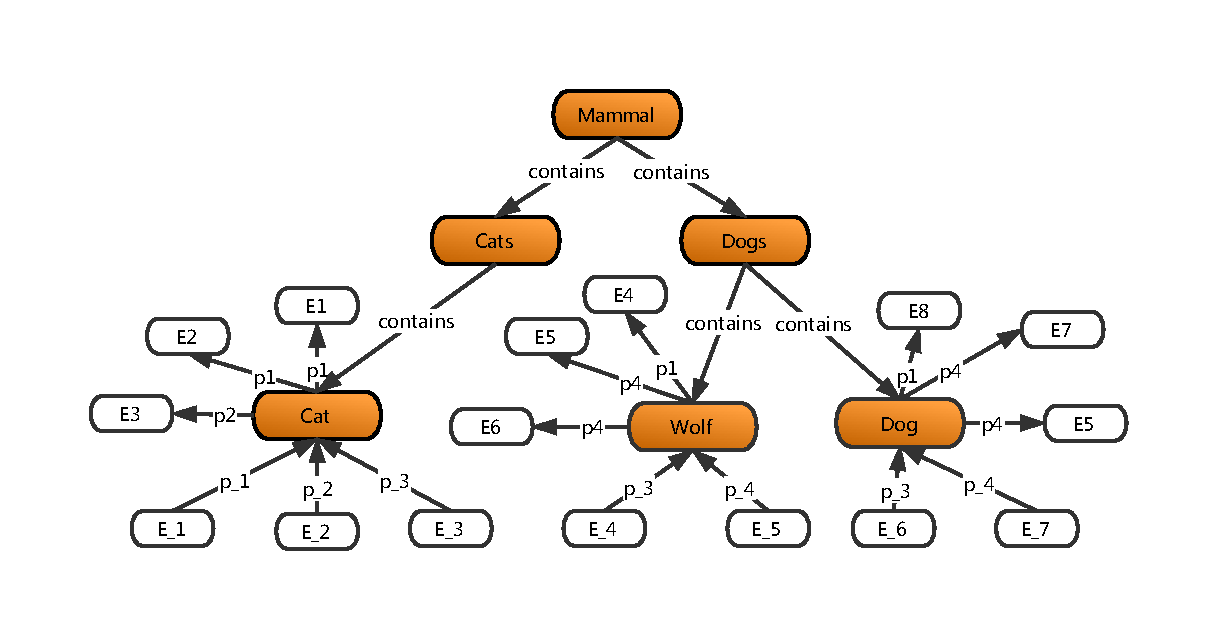
\includegraphics[width=1.1\textwidth]{pic/introduction.pdf}\\
    \caption{Subgraph example in knowledge graph}
    \label{weak1}
\end{figure*}

As show in figure \ref{weak1}, the subgraph contains \emph{Dogs} and \emph{Cats} extracted from
knowledge. We simplify the specific features of \emph{Dogs} and \emph{Cats} to concise symbol shown as $E_i$ in figure. 
We can see that the entity \emph{Cat} plays the role 
of both \emph{Object(Cats contains Cat)} and \emph{Subject(Cat $p_1$ $E_1$)}
in the pattern of triples. The \emph{predicate} which is connected with an entity(Cat)
may be regarded as an outgoing($p_1$) or incoming \emph{predicate}($p_{_1}$).
In the paper\cite{aaai/Pirro12}, the relatedness space for an entity ${E_i}$ is modelled as a 
$k$-dimensional weighted vector \emph{V$_i$}, where each dimension represents
the informativeness of a specific \emph{predicate}.
For example, the weighted vector for \emph{Cat} is 
$[v_{p_1}^o, v_{p_2}^o, v_{p_\_1}^i, v_{p_\_2}^i, v_{p_\_2}^i]$ in which $v_{p_i}^o$ 
means the vector value of outgoing predicate $p_i$ and $v_{p_j}^i$ 
means the vector value of incoming predicate $p_j$.
In this example, from the view of outgoing \emph{predicate} $p_i$, there are three triples
\emph{(Cat $p_1$ $E_1$)}, \emph{(Cat $p_1$ $E_2$)} and \emph{(Cat $p_2$ $E_3$)} which describe the entity \emph{Cat}.
Specifically, in order to compute the vector value of $p_1$,
the way of paper \cite{aaai/Pirro12} in which they got the informativeness of $p_i$ was to count the number
of triples with the form of \emph{(Cat $p_1$ ?)} firstly, then they divided this result
by the total number of triples in which \emph{Cat} appears
((Cat $p_1$ $E_1$), (Cat $p_1$ $E_2$), (Cat $p_2$ $E_3$)), i.e., $v_{p_1}^o$=2/3.
They\cite{aaai/Pirro12} only considered the informativeness of \emph{prediacte},
and ignored the function of a set of specific \emph{objects} in a pattern of triple.
Besides, there is another aspect they have ignored. In this example, for entities $Cat$,
$Dog$ and $Wolf$, let us see the informativeness of prediacte $p_1$. We get
\emph{(Cat $p_1$ $E_1$), (Cat $p_1$ $E_2$), (Wolf $p_1$ $E_4$)} and \emph{(Dog $p_1$ $E_8$)}. 
It is obvious that when they\cite{aaai/Pirro12} computed relatedness between \emph{Cat} and \emph{Wolf}, 
they got the same vector value for predicate $p_1$ both in the aspect of \emph{Wolf} and \emph{Dog}.
In other words, in the dimension of predicate $p_1$ vector between pair (\emph{Cat},\emph{Wolf}) and
(\emph{Cat},\emph{Dog}), they got no difference. Accordingly, they did not distinguish the different
objects for a specific predicate. In order to improve the performance of 
semantic relatedness measurement based on knowledge graph, we propose a threefold model which is shown as follows:

1. For given a pair of words, the first job is to query the corresponding entities. In order to use the
neural network for training the dataset, we also need to construct a graph which contains all related
entities, attributes and relations between the corresponding entity pairs.

2. We use Starspace proposed by Facebook for knowledge graph instead of Word2vec to train the subgraph
extracted from the knowledge graph. Then we can get a distributional representation(vector) for each
entity and predicate. 

3. When we take as inputs a pair of words, we can get two sets of corresponding entities queried from
knowledge graph. Then we can get multiple relatedness scores after a full link between these two sets of entities.
Inspired by \cite{acl/IacobacciPN15}, we utilize an approach to combine the 
relatedness scores as the final semantic relatedness score in knowledge graph.

This paper is organized as follows. We give the related work about semantic relatedness
measurement in section \ref{related-word}. Then we elaborate the threefold model for
computing relatedness scores in section \ref{methodlogy}. Finally, we display detailed
illustrations of experiment results which show that our model outperform the state-of-the-art model.
\section{Related Work}
Computing semantic relatedness(SR) between two elements(words, sentences,
texts etc.) is a fundamental task for many applications in Natural Language
Processing(NLP) such as lexicon induction(\cite{aaai/QadirMGL15}), Named 
Entity Disambiguation{\cite{acl/HanZ10}}, Keyword Extraction
(\cite{ijcai/ZhangFW13}) and Information Retrieval(\cite{acl/GurevychMZ07}). 
Additionaly, computing semantic relatedness contributes other applications, 
for example, opinion spam problem (\cite{www/SandulescuE15}) and so on(+some example). 
In this paper we focus on computing semantic relatedness between two 
words in knowledge graph with neural network.


Semantic measures are mathematical tools used to estimate the strength of the 
semantic relationship between units of language, concepts or instances, through 
a (numerical) description obtained according to the comparison of information 
supporting their meaning. The semantic measures contain semantic relatedness,
semantic similarity, semantic distance. The semantic distance equal to semantic 
unsimilarity. The similarity is only one particular type of relatedness.
Comparison to similarity fails to give a complete view of a relatedness measures.


In this paper we computing semantic relatedness on the account of knowledge
graph. Computational of semantic relatedness is a superset of similarity.
The similarity is only one particular type of relatedness, comparison to
similarity fails to give a complete view of a relatedness measures.

Approaches to measuring semantic relatedness that use lexical
resources (instead of distributional similarity of words, 
e.g. Landauer and Dumais (1997) and Turney (2001)) transform
that resource into a network or graph and compute
relatedness using paths in it. Rada et al. (1989) traverse
MeSH, a term hierarchy for indexing articles in Medline,
and compute semantic relatedness straightforwardly in
terms of the number of edges between terms in the hierarchy.
Jarmasz and Szpakowicz (2003) use the same approach
with Roget’s Thesaurus while Hirst and St-Onge (1998) apply
a similar strategy to WordNet. Since the edge counting
approach relies on a uniform modeling of the hierarchy,
researchers started to develop measures for computing semantic
relatedness which abstract from this problem (Wu and
Palmer, 1994; Resnik, 1995; Leacock and Chodorow, 1998;
Finkelstein et al., 2002; Banerjee and Pedersen, 2003, inter
alia). Those researchers, however, focused on developing
appropriate measures while keeping WordNet as the de facto
primary knowledge source.

\cite{aaai/StrubeP06}
\cite{ijcai/GabrilovichM07}
\cite{www/RadinskyAGM11}

\cite{aaai/Pirro12}
\cite{aaai/NavigliP12}

\cite{acl/IacobacciPN15}

\cite{ijcai/SenJHMOMVWH15} domain specific semantic relatedness 


In this paper we focused on semantic relatedness, which
generalizes similarity by considering not only specialization
relations between words. The application of semantic
relatedness span different areas from natural language processing
(Patwardhan, Banerjee, and Pedersen 2003) to distributed
systems (Pirro, Ruffolo, and Talia 2008). In the Se- ´
8http://relwod.wordpress.com
9http://uniprot.bio2rdf.org/sparql
mantic Web context, some initiatives consider RDF predicates
for vocabulary suggestion (Oren, Gerke, and Decker
2007) while other (Freitas et al. 2011) exploit relatedness
for query answering over Linked Data. However, differently
from REWOrD none of them is specifically focused on computing
relatedness in the Web of Data.
Generally speaking, computational approaches to relatedness
exploit different sources of background knowledge
such as WordNet (e.g., (Resnik 1995; Budanitsky A 2001)),
MeSH (e.g., (Rada, Mili, and Bicknell 1989; Pirro and ´
Euzenat 2010)) or search engines (e.g., (Bollegala, Matsuo,
and Ishizuka 2007; Turney 2001)). Recently, Wikipedia
has been shown to be the most promising source of background
knowledge for relatedness estimation (Gabrilovich
and Markovitch 2007). Therefore we’ll consider approaches
exploiting Wikipedia as baseline for comparison.
WikiRelate! (Ponzetto and Strube 2007), given two words
first retrieves the corresponding Wikipedia articles whose titles
contain the words in input. Then, it estimates relatedness
according to different strategies among which comparing
the texts in the pages or computing the distance between
the Wikipedia categories to which the pages belong.
Explicit Semantic Analysis (Gabrilovich and Markovitch
2007) compute relatedness both between words and text
fragments. ESA derives an interpretation space for concepts
by preprocessing the content of Wikipedia to build
an inverted index that for each word, appearing in the corpus
of Wikipedia articles, contains a weighted list of articles
relevant to that word. Relevance is assessed by the
TFIDF weighting scheme while relatedness is computed by
the cosine of the vectors associated to the texts in input.
WLM (Milne and Witten 2008) instead of exploiting text
in Wikipedia articles, scrutinizes incoming/outgoing links
to/from articles. WikiWalk (Yeh et al. 2009) extends the
WLM by exploiting not only link that appear in an article
(i.e., a Wikipedia page) but all links, to perform a random
walk based on Personalized PageRank.
The most promising approach, in terms of correlation, is
ESA. However, ESA requires a huge preprocessing effort to
build the index, only leverages text in Wikipedia and does
not consider links among articles. Therefore, it may suffer
some problems when the amount of text available is not large
enough to build the interpretation vectors or when changing
the source of background knowledge.
\section{Methodlogy}
\label{methodlogy}
In order to compute semantic relatedness of a pair of words, we propose a model which is
threefold. 
For a given pair of words, we first query the corresponding entities in knowledge graph.
We need to construct a specific graph which contains all related entities and attributes between the 
corresponding entity pairs. Then we use \emph{Starspace}\cite{corr/Ledell17} to train the constructed 
graph. For each entity and relationship, this method produces a representation of vector.
In our method, we use cosine function to compare vectors corresponding to word pairs and get the relatedness scores.
Besides, in the query step, we would get several corresponding entities for an input word. Inspired by
the SenseEmbed\cite{acl/IacobacciPN15}, we combine the relatedness scores computed from the multiple pairs of entities 
as the final measure sorce between two words.

% Please add the following required packages to your document preamble:
% \usepackage{booktabs}
\begin{table*}[]
    \small
    \centering
    \caption{Query Entities (\emph{DBPedia:} equals \emph{http://dbpedia.org/resource/})}
    \label{entities}
    \renewcommand\arraystretch{1.6}
    \setlength{\tabcolsep}{0.8mm}{
    \begin{tabular}{llclc}
    \toprule
    \textbf{Words}  & automobile                                               & \textbf{Refcount} & car                                      & \textbf{Refcount} \\ \hline
    \textbf{Entity} & DBPedia:Automobile                   & 5096     & DBPedia:Automobile   & 5096     \\ \hline
    \textbf{Entity} & DBPedia:Auto\_racing                 & 2885     & DBPedia:NASCAR       & 4317     \\ \hline
    \textbf{Entity} & DBPedia:Ferry                        & 2501     & DBPedia:Tram         & 3988     \\ \hline
    \textbf{Entity} & DBPedia:Internal\_combustion\_engine & 1639     & DBPedia:Auto\_racing & 2885     \\ \hline
    \textbf{Entity} & DBPedia:Gasoline                     & 1486     & DBPedia:Ferry        & 2501     \\ \hline
    \end{tabular}    
    }
\end{table*}

\subsection{Construct graph}
\label{sec:construct graph}
Our aim is to compute the semantic relatedness between a pair of words. The process of relatedness measure
needs complete and ample background knowledge which can be gathered from knowledge graph, such as
DBPedia\footnote{http://wiki.dbpedia.org/}, 
YAGO\footnote{https://www.mpi-inf.mpg.de/departments/databases-and-information-systems/research/yago-naga/yago} etc.
The first problem we face is how to obtain knowledge which is associated with given words from knowledge graph. 
In our model, we utilize the DBPedia as our knowledge base to gather corresponding entities triggered by the given words.
We rely on lookup service\footnote{http://lookup.dbpedia.org/api/search/KeywordSearch} that is provided by DBPedia to achieve this object. 
We use $W_{w_i}$ to denote the set of corresponding entities in knowledge graph when we complete a query by word $w_i$.
Then we get $W_{w_i}=\{E_1,...,E_k\}$ where $E_i$ is the $i_{th}$ query entity associated with the given word.
As show in Table \ref{entities}, for a given word pair \emph{(automobile,car)}, 
we can get the appropriate entities which are described as URIs in DBPedia. 
These URIs describe entities so accurate that we can access knowledge graph using powerful
query language SPARQL\footnote{https://www.w3.org/TR/sparql11-overview/} to get everything we want.

% sparql query norm for graph construction

An entity can be surrounded by entities as well as attributes. There is an example to illustrate this structure
in knowledge graph. Suppose that there is a person \emph{A}, his age is \emph{24}. His name is \emph{"John A"}.
He has a friend called person \emph{B}. This person \emph{B} is an Entity surrounding the \emph{A}.
Then the number \emph{24} and the literal \emph{"John A"} are not entities in knowledge graph,
but all are the attributes surrounding this person \emph{A}.
We can use the URIs shown in table\ref{entities} to access knowledge graph with the help of SPARQL. Next we need to construct a subgraph 
that contains all related entities, attributes and relations between the corresponding entity pairs. Inspired by BabelRelate!\cite{aaai/NavigliP12},
we propose a modified method to get our semantic subgraph. We get query sets of entities $W_{w_1}$ and $W_{w_2}$ individually
by words $w_1$ and $w_2$. Then we select the subgraph which contains all the paths which connect entities in
$ENT = W_{w_1} \cup W_{w_1}$. Besides, this subgraph also contains all attributes for each entity in $ENT$. We do 
this by building a directed graph ${G = (V, E)}$ which contains all relevant information which describes
the entities set.

i) We define the set $V$ in $G$ as $V:=ENT$ first. 
The size of set $V$ is not fixed. It would be extended in the following steps.
As for the set $E$, we initialize it as empty, i.e., $E:=\emptyset$.

ii)The goal of our method is to get the precise vector representations for entities,
that requires more complete information which surround the entities.
Accordingly, for a specific entity, we not only need to consider its neighbor entities or attributes, but also
need to find all paths which connect the nodes in $V$. 
It is known to all, the shorter length of paths between two entities, the more relative these entities are.
We firstly get the one-hop neighbors for each $v \in V$. 
Secondly, we adopt Depth-First Search(DFS) to go through the knowledge graph. Every time we find a node
$v^{'} \in V$ but $v \ne v^{'}$ along a path($v, v_1, v_2,...,v_n, v^{'}$), we add all intermedia 
nodes and edges in this path to $G$, i.e., $V:=V \cup \{v_1, ..., v_n\}$, 
$E:=E \cup \{(v, v_1), ..., (v_n, v^{'})\}$.

iii) Next, we get all relevant attributes which are described as literal, number or something 
else special symbol in knowledge graph. For one entity $v_i \in V$, we collect all the one-hop attributes 
$\{a_1, a_2, ..., a_k\}$. Then we have $V:=V \cup \{a_1, ..., a_k\}$ and
$E:=E \cup \{(v_i, a_1), ..., (v_i, a_k)\}$ ($v_i \in V$).

By this way, we extract a subgraph from DBPedia which consists of the relevant information which describes
the pair of entities.

\subsection{Embedding for Subgraph}
\label{sec:train}
The constructed graph is fundamentally a multi-relational graph in which an entity is described by a set of discrete
\emph{entities} and \emph{attributes}. Fortunately, there have been an excellent work proposed by Facebook AI Research,
\emph{StarSpace}\cite{corr/Ledell17}. The model works by embedding those entities comprised of discrete features and
comparing them against each other. In this section, we introduce the basic contents of \emph{StarSpace} briefly and 
elaborate how we utilize this model to get the vector representation of entities and relations. \emph{StarSpace} is available as
an open-source project at github\footnote{https://github.com/facebookresearch/StarSpace}.

In \emph{StarSpace}, to train our model, we need to compare entities which are described by a set of discrete
\emph{entities} and \emph{attributes}. Specially, there is the following loss function in $StarSpace$:

\begin{small}
    \begin{equation}
        \nonumber
        \label{starspace_formula}
        \sum_{\substack{(a,b) \in V^+\\ b^- \in V^-}}L^{batch}(sim(a,b),sim(a,b_1^-),...,sim(a,b_k^-))
    \end{equation}
\end{small}
In our problem, the input data is a graph of $(h, r, t)$ triples, consisting of a head entity $h$, 
a relation $r$ and a tail entity $t$.
Following the original paper which describes $StarSpace$, there are several explanations for this loss function:

1) The positive entity pair (a,b) comes from the set $V^+$ sampled from constructed graph $G$. 
In our problem, the input is a group of triples $(h, r, t)$. In order to make our input fit
the sample batch $(a, b)$, we need to select uniformly at random to get positive sample $V^+$ in two strategies:
(i)$a$ consists of the bag of features $h$ and $r$, while $b$ consists only of $t$; 
(ii)$a$ consists of $h$, and $b$ consists of $r$ and $t$. 

2) Negative entities $b^-$ are sampled from the set of possible entities $V^-$.  
StarSpace utilizes a $k$-negative sampling strategy\cite{corr/Mikolov13} to select $k$ negative pairs for each batch update. 
They select randomly whithin the set of entities that can appear in the second argument of the similarity function.

3) The selection of function $sim(.,.)$ is designed as a hyper-parameter: cosine similarity and inner product.
In our problem, we adopt cosine similarity for the model as the cosine works better than inner product for
larger dataset. This situation is mentioned in the paper of StarSpace.

4) The loss function $L_{batch}$ compares the positive pairs $(a,b)$ with the negative pairs $(a, b_i^-)$, $i=1,...,k$.
It is also optional between margin ranking loss and negative log loss of softmax. All experiments in $StarSpace$ show
the former performed on par or better. Thus we use margin ranking loss as our loss function for computing semantic relatedness.

5) The method optimization inherit the strategy of stochastic gradient descent(SGD) used in $Starspace$. Each SGD step is one
sampling from $V^+$ in the outer sum.

As a result, we take the constructed graph $G$ of $(h, r, t)$ triples as inputs for the training model.
For each entity and relation in graph $G$, there is a fixed-length vector which can
then be used to compute semantic relatedness via cosine function.

%(Experiments:K-sample,dim of vector,epochs)
% \cite{aaai/BordesWCB11}


\subsection{Semantic Relatedness Measure}
\label{sec:measure}
For a given pair of words($w_m$, $w_n$), we get ($W_{w_m}$, $W_{w_n}$), and $W_{w_m}=\{E_m^1,E_m^2...,E_m^k\}$,
$W_{w_n}=\{E_n^1,E_n^2,...,E_n^k\}$. Then for each entity $E_m^i$ in $W_{w_m}$, we will get learnt embedding vector
$\overrightarrow E_m^i$.
Note that, there might be different number of entities associated with the given
word. We just consider the top-$k$ entities in each entities set. An analysis of the impact of $k$ is
given in section of experiments.

For a pair ($w_1$, $w_2$), we compute semantic relatedness between their corresponding entities. After that, we
get $k*k$ relatedness results where $k$ is number of entities queried from knowledge graph.
The task which combines multiple semantic measurement is similar with the work in SenseEmbed\cite{acl/IacobacciPN15}.
The author captureed the different meanings of a word and transformed word embedding to the sense level.
They utilized the weighted combination of comparison in sense level which achieved a high correlation coefficient.
In our work, the multiple-pair entities produce different semantic measurement. Traditional work only considers the
the relatedness measurement of closest objects. If we only utilize closest combination, the contributions of the other
entities would be ignored. Following the work in SenseEmbed, we combine all those relatedness
results reasonably to get more human-like measurement.

1) For two entities $E_1$ and $E_2$, we utilize cosine function to compute the
distance between two embedding vectors($\overrightarrow E_1$, $\overrightarrow E_2$):

\begin{small}
    \begin{equation}
        \label{cos}
        \nonumber
        Cos(\overrightarrow E_1,\overrightarrow E_2) = \frac{\overrightarrow E_1 \cdot 
        \overrightarrow E_2}{\left \| \overrightarrow E_1 \right \|\left \| \overrightarrow E_2 \right \|}
    \end{equation}
\end{small}

2) Following SenseEmbed, we take two strategies to compute semantic relatedness between given
words $w_1$ and $w_2$ for comparison. One is conventional approach \cite{BudanitskyH06} which considers just the closest entities
among multiple vector pairs. There are $W_{w_1}$ and $W_{w_2}$ represent two entities sets associated with two
input words $w_1$ and $w_2$. $\overrightarrow E_i$ is the learnt embedding vector of entity $E_i$. We can get the
formalization for this strategy.

\begin{small}
    \begin{equation}
        \label{cos}
        \nonumber
        Rel_{closest}(w_1, w_2) = \max \limits_{\substack{E_1 \in W_{w_1} \\ E_2 \in W_{w_1}}}
        Cos(\overrightarrow E_1,\overrightarrow E_2)
    \end{equation}
\end{small}
However this relatedness measurement approach misses contributions of the other entities.
In fact, psychological studies suggest that humans, while comparing similarity between a pair of words, consider
different meanings of two words but not only the closest pairs\cite{Tversky77}. This claim can be directly popularized to compute
relatedness between words. There usually are various meanings for a single word. Analogously we can query multiple
entities associated with the word from knowledge graph. Only consider the entities pair which have the closest distance
would not be conforming with the way of human thinking.

There is another strategy for computing semantic relatedness, called \emph{weighted}, in which
we consider the contributions of different entities associated with given words. The contributions are
scaled according to how they relative to the words. Fortunately, the lookup services of DBPedia can
return a list of ranked DBpedia resources for a search string or a single word. There is a specific label called
$Refcount$ that count the number of Wikipedia page inlinks for a resource. This number is required for ranking.
We can utilize this number to estimate the dominance of each specific entity resource in knowledge graph.
To this end, we use an operation of normalization. For each entity $E \in W_{w_i}$, we get the dominance of
$E$ by dividing the value of $Refcount$ by the sum of all $Refcount$ value of entities in  $W_{w_i}$:

\begin{small}
    \begin{equation}
        \label{cos}
        \nonumber
        d(E) = \frac{refcount(E)}{\sum_{{E}'\in W_i} refcount({E}')}
    \end{equation}
\end{small}

Besides, those entities which are closer would play a more important role in computing semantic relatedness.
Following the SenseEmbed, we model this by biasing the relatedness computation towards closer entities through a power function with
parameter $\alpha$. The relatedness of a pair of words $w_1$ and $w_2$ is computed by using $weighted$ strategy:

\begin{small}
    \begin{equation}
        \begin{split}
        \label{cos}
        \nonumber
        Rel_{weight}&(w_1, w_2)=\\ 
        &\sum_{E_1 \in W_1}\sum_{E_2 \in W_2}d(E_1)d(E_2)Cos(\overrightarrow E_1,\overrightarrow E_2)^\alpha 
        \end{split}
    \end{equation}
\end{small}

In this strategy, we given the entity pairs which is closer a more important role to determine the final semantic relatedness
score. Experiments in below show that the $weighted$ strategy outperforms the $closest$.
% \begin{small}
%     \begin{math}
%         \label{cos}
%         \nonumber
%         Dis(E_1,E_2)
%         =\lambda Cos(\overrightarrow E_1,\overrightarrow E_2) + (1-\lambda)\frac{1}{path(E_1, E_2)}
%     \end{math}
% \end{small}


% \begin{small}
%     \begin{equation}
%         \label{cos}
%         \nonumber
%         Cos^*(\overrightarrow E_1,\overrightarrow E_2)=
%         \begin{cases} 
%         Cos(\overrightarrow E_1,\overrightarrow E_2) \times \beta, &if(s_1, s_2) \in E\\
%         Cos(\overrightarrow E_1,\overrightarrow E_2) \times \beta^{-1}, &otherwise
%         \end{cases}
%     \end{equation}
% \end{small}
\section{Template}

\subsection{Semantic Measure}
1. Semantic relatedness, which computes the correlation degree of two objects such as
words, entities and texts, is fundamentalfor many applications. It has long been thought
that when human measure the relatedness between a pair of owrds, a deeper reasoning is 
triggered to compare the concepts behind the words.
While many traditional studies on semantic relatedness utilize the lexical databases, 
such as WordNet or Wikitionary, the recent word embedding learning approaches 
demonstrate their abilities to capture syntactic and semantic information, and 
outperform the lexicon-based methods. 

2. Despite the well-established technical distinction between semantic similarity and 
relatedness (Agirre et al., 2009; Budanitsky and Hirst, 2006; Resnik, 1995), comparison
to established similarity norms from psychology remains part of the standard evaluative 
procedure for assessing computational measures of semantic relatedness. Because similarity 
is only one particular type of relatedness, comparison to similarity norms fails to give 
a complete view of a relatedness measure’s efficacy.

3. Semantic relatedness indicates how much two concepts are
related in a taxonomy by using all relations between them
(i.e. hyponymic/hypernymic, meronymic and any kind of
functional relations including has-part, is-made-of, is-anattribute-of,
etc.). When limited to hyponymy/hyperonymy
(i.e. is-a) relations, the measure quantifies semantic similarity
instead. Semantic relatedness measures are used in many
applications in Natural Language Processing (NLP) such as
word sense disambiguation (Patwardhan et al., 2005), information
retrieval (Finkelstein et al., 2002), interpretation of
noun compounds and spelling correction.

4. Computing semantic relatedness between two words (or
texts) is a fundamental task in natural language processing,
artificial intelligence and information retrieval. Strictly
speaking, semantic relatedness is a more general notion than
semantic similarity as it captures not only closeness between
two objects within a type hierarchy (e.g., river and stream),
but also any other relations (e.g., river and boat) (Budanitsky
and Hirst 2006). Traditionally, semantic similarity has
been computed either within some lexicon (Jarmasz 2003;
Resnik 1995; Jiang and Conrath 1997; Lin 1998) or by comparing
the distributional properties of contexts (Deerwester
et al. 1990; Gabrilovich and Markovitch 2007; Hassan and
Mihalcea 2011). On the other hand, semantic relatedness
has been largely modeled by co-occurrences within a window
in a large text corpus.

5. Reasoning about semantic relatedness of natural language uttrances is routinely performed by 
humans but remains an unsurmountable obstacle for computers. Humans do not judge tex relatedness
merely at the level of text words. Words trigger reasoning at a much deeper level that manipulates
concept--the basic units of meaning that serve humans to organize and share their knowledge. Thus, 
humans interpret the specific wording of a documemnt in the much larger context of their background 
knowledge and experimence.

It has long been recognized that in order to process natural language, computers require access to 
vast amounts of common-sense and domain-specific world knowledge. However, prior work on semantic 
relatedness was based on purely statistical techniques that did not make use of background
knowledge or on lexical resources that incorporate very limited knowledge about the world.

\subsection{Knowledge graph} 
1. Knowledge graphs encode structured information of entities and their rich relations.
Although a typical knowledge graph may contain millions of entities and billions of 
relational facts, it is usually far from complete.

2.People build large-scale knowledge graphs (KG), such as Freebase, DBpedia and YAGO, 
to store complex structured information about the facts of the real world. The facts
in KGs are usually organized in the form of triplets, e.g., (Washington, CapitalOf, USA). 
KGs have been widely adoptedin various applications such as question answering and Web search.

Existing KGs have already included thousands of relation
types, millions of entities and billions of triplets. Nevertheless
these KGs remain far from complete as compared to the
amount of real-world facts. In order to further expand KGs,
many researches have been devoted to automated fact exploration.

Recently, neural-based representation learning (RL) methods
are proposed to encode the semantics of both entities
and relations in low-dimensional semantic space (i.e., embeddings),
which can be further employed to discover novel facts.

3. 


\subsection{Knowledge graph embedding}
1. Recently, models such as TransE and TransH build entity and relation embeddings by 
regarding a relation as translation from head entity to tail entity. In fact, an entity
may have multiple aspects and various relations may focus on different aspects of
entities, which makes a common space insufficient for modeling.

\subsection{Random walking}
A number of aggregated proximity measures based on random walk have been proposed in the 
literature, such as PageRank (including Personalized PageRank) and hitting time. Previous
studied showed that these aggregated measures are more effective than individual links 
and paths.

\subsection{applications of sr}
information extraction
semantic analysis
understanding the meaning of phrase

\section{General Instructions}

Manuscripts must be in two-column format.  Exceptions to the
two-column format include the title, authors' names and complete
addresses, which must be centered at the top of the first page, and
any full-width figures or tables (see the guidelines in
Subsection~\ref{ssec:first}). \textbf{Type single-spaced.}  Start all
pages directly under the top margin. See the guidelines later
regarding formatting the first page.  The manuscript should be
printed single-sided and its length
should not exceed the maximum page limit described in Section~\ref{sec:length}.
Pages are numbered for  initial submission. However, \textbf{do not number the pages in the camera-ready version}.

By uncommenting {\verb|\aclfinalcopy|} at the top of this 
 document, it will compile to produce an example of the camera-ready formatting; by leaving it commented out, the document will be anonymized for initial submission.  When you first create your submission on softconf, please fill in your submitted paper ID where {\verb|***|} appears in the {\verb|\def\aclpaperid{***}|} definition at the top.

The review process is double-blind, so do not include any author information (names, addresses) when submitting a paper for review.  
However, you should maintain space for names and addresses so that they will fit in the final (accepted) version.  The ACL 2018 \LaTeX\ style will create a titlebox space of 6.35 cm for you when {\verb|\aclfinalcopy|} is commented out.  

\subsection{The Ruler}
The ACL 2018 style defines a printed ruler which should be present in the
version submitted for review.  The ruler is provided in order that
reviewers may comment on particular lines in the paper without
circumlocution.  If you are preparing a document without the provided
style files, please arrange for an equivalent ruler to
appear on the final output pages.  The presence or absence of the ruler
should not change the appearance of any other content on the page.  The
camera ready copy should not contain a ruler. (\LaTeX\ users may uncomment the {\verb|\aclfinalcopy|} command in the document preamble.)  

\textbf{Reviewers}: note that the ruler measurements do not align well with
lines in the paper -- this turns out to be very difficult to do well
when the paper contains many figures and equations, and, when done,
looks ugly. In most cases one would expect that the approximate
location will be adequate, although you can also use fractional
references ({\em e.g.}, the first paragraph on this page ends at mark $117.5$).

\subsection{Electronically-available resources}

ACL provides this description in \LaTeX2e{} ({\small\tt acl2018.tex}) and PDF
format ({\small\tt acl2018.pdf}), along with the \LaTeX2e{} style file used to
format it ({\small\tt acl2018.sty}) and an ACL bibliography style ({\small\tt acl\_natbib.bst})
and example bibliography ({\small\tt acl2018.bib}).
These files are all available at
\url{http://acl2018.org/downloads/acl18-latex.zip}.

A Microsoft Word template file ({\small\tt acl18-word.docx}) and example submission pdf ({\small\tt acl18-word.pdf})
is available at
\url{http://acl2018.org/downloads/acl18-word.zip}.
We strongly recommend the use of these style files, which have been
appropriately tailored for the ACL 2018 proceedings.

\subsection{Format of Electronic Manuscript}
\label{sect:pdf}

For the production of the electronic manuscript you must use Adobe's
Portable Document Format (PDF). PDF files are usually produced from
\LaTeX\ using the \textit{pdflatex} command. If your version of
\LaTeX\ produces Postscript files, you can convert these into PDF
using \textit{ps2pdf} or \textit{dvipdf}. On Windows, you can also use
Adobe Distiller to generate PDF.

Please make sure that your PDF file includes all the necessary fonts
(especially tree diagrams, symbols, and fonts with Asian
characters). When you print or create the PDF file, there is usually
an option in your printer setup to include none, all or just
non-standard fonts.  Please make sure that you select the option of
including ALL the fonts. \textbf{Before sending it, test your PDF by
  printing it from a computer different from the one where it was
  created.} Moreover, some word processors may generate very large PDF
files, where each page is rendered as an image. Such images may
reproduce poorly. In this case, try alternative ways to obtain the
PDF. One way on some systems is to install a driver for a postscript
printer, send your document to the printer specifying ``Output to a
file'', then convert the file to PDF.

It is of utmost importance to specify the \textbf{A4 format} (21 cm
x 29.7 cm) when formatting the paper. When working with
{\tt dvips}, for instance, one should specify {\tt -t a4}.
Or using the command \verb|\special{papersize=210mm,297mm}| in the latex
preamble (directly below the \verb|\usepackage| commands). Then using 
{\tt dvipdf} and/or {\tt pdflatex} which would make it easier for some.

Print-outs of the PDF file on A4 paper should be identical to the
hardcopy version. If you cannot meet the above requirements about the
production of your electronic submission, please contact the
publication chairs as soon as possible.

\subsection{Layout}
\label{ssec:layout}

Format manuscripts two columns to a page, in the manner these
instructions are formatted. The exact dimensions for a page on A4
paper are:

\begin{itemize}
\item Left and right margins: 2.5 cm
\item Top margin: 2.5 cm
\item Bottom margin: 2.5 cm
\item Column width: 7.7 cm
\item Column height: 24.7 cm
\item Gap between columns: 0.6 cm
\end{itemize}

\noindent Papers should not be submitted on any other paper size.
 If you cannot meet the above requirements about the production of 
 your electronic submission, please contact the publication chairs 
 above as soon as possible.

\subsection{Fonts}

For reasons of uniformity, Adobe's \textbf{Times Roman} font should be
used. In \LaTeX2e{} this is accomplished by putting

\begin{quote}
\begin{verbatim}
\usepackage{times}
\usepackage{latexsym}
\end{verbatim}
\end{quote}
in the preamble. If Times Roman is unavailable, use \textbf{Computer
  Modern Roman} (\LaTeX2e{}'s default).  Note that the latter is about
  10\% less dense than Adobe's Times Roman font.

\begin{table}[t!]
\begin{center}
\begin{tabular}{|l|rl|}
\hline \bf Type of Text & \bf Font Size & \bf Style \\ \hline
paper title & 15 pt & bold \\
author names & 12 pt & bold \\
author affiliation & 12 pt & \\
the word ``Abstract'' & 12 pt & bold \\
section titles & 12 pt & bold \\
subsection titles & 11 pt & bold \\
document text & 11 pt  &\\
captions & 11 pt & \\
abstract text & 11 pt & \\
bibliography & 10 pt & \\
footnotes & 9 pt & \\
\hline
\end{tabular}
\end{center}
\caption{\label{font-table} Font guide. }
\end{table}

\subsection{The First Page}
\label{ssec:first}

Center the title, author name(s), and affiliation(s) across both
columns (or, for the initial submission, \textbf{Anonymous ACL submission} for names and affiliations). Do not use footnotes for affiliations. 
Include the paper ID number assigned during the submission process in the header. 
Use the two-column format only when you begin the abstract.

\textbf{Title}: Place the title centered at the top of the first page, in
a 15-point bold font. (For a complete guide to font sizes and styles,
see Table~\ref{font-table}) Long titles should be typed on two lines
without a blank line intervening. Approximately, put the title at 2.5
cm from the top of the page, followed by a blank line, then the
author name(s), and the affiliation(s) on the following line. Do not
use only initials for given names (middle initials are allowed). Do
not format surnames in all capitals ({\em e.g.}, use ``Mitchell'' not
``MITCHELL'').  Do not format title and section headings in all
capitals as well except for proper names (such as ``BLEU'') that are
conventionally in all capitals.  The affiliation should contain the
author's complete address, and if possible, an electronic mail
address. Start the body of the first page 7.5 cm from the top of the
page.

The title, author names and addresses should be completely identical
to those entered to the electronic paper submission website in order
to maintain the consistency of author information among all
publications of the conference. If they are different, the publication
chairs may resolve the difference without consulting with you; so it
is in your own interest to double-check that the information is
consistent.

\textbf{Abstract}: Type the abstract at the beginning of the first
column. The width of the abstract text should be smaller than the
width of the columns for the text in the body of the paper by about
0.6 cm on each side. Center the word \textbf{Abstract} above the body of the abstract using the font size and style shown in Table~\ref{font-table}. The abstract should be a concise
summary of the general thesis and conclusions of the paper. It should
be no longer than 200 words. The font size of the abstract text should be as shown in Table~\ref{font-table}. 

\textbf{Text}: Begin typing the main body of the text immediately after
the abstract, observing the two-column format as shown in 
the present document. 
Do not include page numbers in the final version.

\textbf{Indent}: Indent when starting a new paragraph, about 0.4 cm.

%Use 11 points for text and subsection headings, 12 points for section headings and 15 points for the title. 


\begin{table}
\centering
\small
\begin{tabular}{cc}
\begin{tabular}{|l|l|}
\hline
\textbf{Command} & \textbf{Output}\\\hline
\verb|{\"a}| & {\"a} \\
\verb|{\^e}| & {\^e} \\
\verb|{\`i}| & {\`i} \\ 
\verb|{\.I}| & {\.I} \\ 
\verb|{\o}| & {\o} \\
\verb|{\'u}| & {\'u}  \\ 
\verb|{\aa}| & {\aa}  \\\hline
\end{tabular} & 
\begin{tabular}{|l|l|}
\hline
\textbf{Command} & \textbf{ Output}\\\hline
\verb|{\c c}| & {\c c} \\ 
\verb|{\u g}| & {\u g} \\ 
\verb|{\l}| & {\l} \\ 
\verb|{\~n}| & {\~n} \\ 
\verb|{\H o}| & {\H o} \\ 
\verb|{\v r}| & {\v r} \\ 
\verb|{\ss}| & {\ss} \\\hline
\end{tabular}
\end{tabular}
\caption{Example commands for accented characters, to be used in, {\em e.g.}, \BibTeX\ names.}\label{tab:accents}
\end{table}

\subsection{Sections}

\textbf{Headings}: Type and label section and subsection headings in the
style shown on the present document.  Use numbered sections (Arabic
numerals) in order to facilitate cross references. Number subsections
with the section number and the subsection number separated by a dot, in Arabic numerals. 
Do not number subsubsections ({\em i.e.}, use \verb|\subsubsection*| instead of \verb|\subsubsection|).

\begin{table*}
\centering
\begin{tabular}{lll}
  output & natbib & previous ACL style files\\
  \hline
  \citep{Gusfield:97} & \verb|\citep| & \verb|\cite| \\
  \citet{Gusfield:97} & \verb|\citet| & \verb|\newcite| \\
  \citeyearpar{Gusfield:97} & \verb|\citeyearpar| & \verb|\shortcite| \\
\end{tabular}
\caption{Citation commands supported by the style file.
  The citation style is based on the natbib package and
  supports all natbib citation commands.
  It also supports commands defined in previous ACL style files
  for compatibility.
  }
\end{table*}

\textbf{Citations}: Citations within the text appear in parentheses
as~\cite{Gusfield:97} or, if the author's name appears in the text
itself, as Gusfield~\shortcite{Gusfield:97}.
Using the provided \LaTeX\ style, the former is accomplished using
{\verb|\cite|} and the latter with {\verb|\shortcite|} or {\verb|\newcite|}.
Collapse multiple citations as in~\cite{Gusfield:97,Aho:72}; this is accomplished with the provided style using commas within the {\verb|\cite|} command, {\em e.g.}, {\verb|\cite{Gusfield:97,Aho:72}|}.  
Append lowercase letters to the year in cases of ambiguities.  
 Treat double authors as
in~\cite{Aho:72}, but write as in~\cite{Chandra:81} when more than two
authors are involved. 
%Collapse multiple citations as
%in~\cite{Gusfield:97,Aho:72}. 

Also refrain from using full citations
as sentence constituents.
%\penalty -5000
We suggest that instead of
\begin{quote}
  ``\cite{Gusfield:97} showed that ...''
\end{quote}
you use
\begin{quote}
``Gusfield \shortcite{Gusfield:97}   showed that ...''
\end{quote}

If you are using the provided \LaTeX{} and Bib\TeX{} style files, you
can use the command \verb|\citet| (cite in text)
to get ``author (year)'' citations.

You can use the command \verb|\citealp| (alternative cite without 
parentheses) to get ``author year'' citations (which is useful for 
using citations within parentheses, as in \citealp{Gusfield:97}).

If the Bib\TeX{} file contains DOI fields, the paper
title in the references section will appear as a hyperlink
to the DOI, using the hyperref \LaTeX{} package.
To disable the hyperref package, load the style file
with the \verb|nohyperref| option:
\verb|\usepackage[nohyperref]{acl2018}|.

\textbf{Compilation Issues}: Some of you might encounter the following error during compilation: 

``{\em \verb|\pdfendlink| ended up in different nesting level than \verb|\pdfstartlink|.}''

This happens when \verb|pdflatex| is used and a citation splits across a page boundary. To fix this, disable the \verb|hyperref| package (see above), recompile and see the problematic citation.
Next rewrite that sentence containing the citation. (See, {\em e.g.}, {\small\tt http://tug.org/errors.html})

\textbf{Digital Object Identifiers}:  As part of our work to make ACL
materials more widely used and cited outside of our discipline, ACL
has registered as a CrossRef member, as a registrant of Digital Object
Identifiers (DOIs), the standard for registering permanent URNs for
referencing scholarly materials. We are requiring all
camera-ready references to contain the appropriate DOIs (or as a
second resort, the hyperlinked ACL Anthology Identifier) to all cited
works.  Thus, please ensure that you use Bib\TeX\ records that contain
DOI or URLs for any of the ACL materials that you reference.
Appropriate records should be found for most materials in the current
ACL Anthology at \url{http://aclanthology.info/}.

As examples, we cite \cite{P16-1001} to show you how papers with a DOI
will appear in the bibliography.  We cite \cite{C14-1001} to show how
papers without a DOI but with an ACL Anthology Identifier will appear
in the bibliography.  

As reviewing will be double-blind, the submitted version of the papers
should not include the authors' names and affiliations. Furthermore,
self-references that reveal the author's identity, {\em e.g.},
\begin{quote}
``We previously showed \cite{Gusfield:97} ...''  
\end{quote}
should be avoided. Instead, use citations such as 
\begin{quote}
``\citeauthor{Gusfield:97} \shortcite{Gusfield:97}
previously showed ... ''
\end{quote}

\textbf{Please do not use anonymous citations} and do not include
acknowledgments when submitting your papers. Papers that do not
conform to these requirements may be rejected without review.

\textbf{References}: Gather the full set of references together under
the heading \textbf{References}; place the section before any Appendices,
unless they contain references. Arrange the references alphabetically
by first author, rather than by order of occurrence in the text.
Provide as complete a citation as possible, using a consistent format,
such as the one for {\em Computational Linguistics\/} or the one in the 
{\em Publication Manual of the American 
Psychological Association\/}~\cite{APA:83}.  Use of full names for
authors rather than initials is preferred.
A list of abbreviations for common computer science journals can be found in the ACM {\em Computing Reviews\/}~\cite{ACM:83}.

The \LaTeX{} and Bib\TeX{} style files provided roughly fit the
American Psychological Association format, allowing regular citations, 
short citations and multiple citations as described above.

\textbf{Appendices}: Appendices, if any, directly follow the text and the
references (but see above).  Letter them in sequence and provide an
informative title: \textbf{Appendix A. Title of Appendix}.

\subsection{Footnotes}

\textbf{Footnotes}: Put footnotes at the bottom of the page and use the footnote font size shown in Table~\ref{font-table}. They may be numbered or referred to by asterisks or other
symbols.\footnote{This is how a footnote should appear.} Footnotes
should be separated from the text by a line.\footnote{Note the line
separating the footnotes from the text.}

\subsection{Figures and Tables}

%\textbf{Placement}: Place figures and tables in the
%paper near where they are first discussed if
%possible.  
%Wide figures and tables may run across both columns and should be placed at the top of a page.

\textbf{Placement}: Place figures and tables in the paper near where they are first discussed, as close as possible to the top of their respective column.

%Color illustrations are discouraged, unless you have verified that  
%they will be understandable when printed in black ink.

\textbf{Captions}: Provide a caption for every illustration; number each one
sequentially in the form:  ``Figure 1: Caption of the Figure.'' ``Table 1:
Caption of the Table.''  Type the captions of the figures and 
tables below the body, using the caption font size shown in Table~\ref{font-table}.

\subsection{Equation}
\label{ssec:eqn}

An example equation is shown below:
\begin{equation}
A=\pi r^2
\end{equation}

The numbering (if any) and alignment of the equations will be done automatically (using \verb|align| or \verb|equation|).

\subsection{Accessibility}
\label{ssec:accessibility}

In an effort to accommodate the color-blind (as well as those printing
to paper), grayscale readability for all accepted papers will be
encouraged.  Color is not forbidden, but authors should ensure that
tables and figures do not rely solely on color to convey critical
distinctions.
A simple criterion: All curves and points in your figures should be clearly distinguishable without color.
%Here we give a simple criterion on your colored figures, if your paper has to be printed in black and white, then you must assure that every curves or points in your figures can be still clearly distinguished.

% Min: no longer used as of ACL 2017, following ACL exec's decision to
% remove this extra workflow that was not executed much.
% BEGIN: remove
%% \section{XML conversion and supported \LaTeX\ packages}

%% Following ACL 2014 we will also we will attempt to automatically convert 
%% your \LaTeX\ source files to publish papers in machine-readable 
%% XML with semantic markup in the ACL Anthology, in addition to the 
%% traditional PDF format.  This will allow us to create, over the next 
%% few years, a growing corpus of scientific text for our own future research, 
%% and picks up on recent initiatives on converting ACL papers from earlier 
%% years to XML. 

%% We encourage you to submit a ZIP file of your \LaTeX\ sources along
%% with the camera-ready version of your paper. We will then convert them
%% to XML automatically, using the LaTeXML tool
%% (\url{http://dlmf.nist.gov/LaTeXML}). LaTeXML has \emph{bindings} for
%% a number of \LaTeX\ packages, including the ACL 2017 stylefile. These
%% bindings allow LaTeXML to render the commands from these packages
%% correctly in XML. For best results, we encourage you to use the
%% packages that are officially supported by LaTeXML, listed at
%% \url{http://dlmf.nist.gov/LaTeXML/manual/included.bindings}
% END: remove

\section{Translation of non-English Terms}

It is also advised to supplement non-English characters and terms
with appropriate transliterations and/or translations
since not all readers understand all such characters and terms.
Inline transliteration or translation can be represented in
the order of: original-form transliteration ``translation''.

\section{Length of Submission}
\label{sec:length}

The ACL 2018 main conference accepts submissions of long papers and
short papers.
 Long papers may consist of up to eight (8) pages of
content plus unlimited pages for references. Upon acceptance, final
versions of long papers will be given one additional page -- up to nine (9)
pages of content plus unlimited pages for references -- so that reviewers' comments
can be taken into account. Short papers may consist of up to four (4)
pages of content, plus unlimited pages for references. Upon
acceptance, short papers will be given five (5) pages in the
proceedings and unlimited pages for references. 

For both long and short papers, all illustrations and tables that are part
of the main text must be accommodated within these page limits, observing
the formatting instructions given in the present document. Supplementary
material in the form of appendices does not count towards the page limit.

However, note that supplementary material should be supplementary
(rather than central) to the paper, and that reviewers may ignore
supplementary material when reviewing the paper (see Appendix
\ref{sec:supplemental}). Papers that do not conform to the specified
length and formatting requirements are subject to be rejected without
review.

Workshop chairs may have different rules for allowed length and
whether supplemental material is welcome. As always, the respective
call for papers is the authoritative source.

\section*{Acknowledgments}

The acknowledgments should go immediately before the references.  Do not number the acknowledgments section ({\em i.e.}, use \verb|\section*| instead of \verb|\section|). Do not include this section when submitting your paper for review.

% include your own bib file like this:
%\bibliographystyle{acl}
%\bibliography{acl2018}
\bibliography{acl2018}
\bibliographystyle{acl_natbib}

\appendix

\section{Supplemental Material}
\label{sec:supplemental}
ACL 2018 also encourages the submission of supplementary material
to report preprocessing decisions, model parameters, and other details
necessary for the replication of the experiments reported in the 
paper. Seemingly small preprocessing decisions can sometimes make
a large difference in performance, so it is crucial to record such
decisions to precisely characterize state-of-the-art methods.

Nonetheless, supplementary material should be supplementary (rather
than central) to the paper. \textbf{Submissions that misuse the supplementary 
material may be rejected without review.}
Essentially, supplementary material may include explanations or details
of proofs or derivations that do not fit into the paper, lists of
features or feature templates, sample inputs and outputs for a system,
pseudo-code or source code, and data. (Source code and data should
be separate uploads, rather than part of the paper).

The paper should not rely on the supplementary material: while the paper
may refer to and cite the supplementary material and the supplementary material will be available to the
reviewers, they will not be asked to review the
supplementary material.

Appendices ({\em i.e.} supplementary material in the form of proofs, tables,
or pseudo-code) should come after the references, as shown here. Use
\verb|\appendix| before any appendix section to switch the section
numbering over to letters.

\section{Multiple Appendices}
\dots can be gotten by using more than one section. We hope you won't
need that.

\end{document}
